\section{Experiment}

\begin{frame}{Experiment}

Goal: test if DISHTINY scheme selects for higher-order individuality

\pause

Use two-level scheme.

\end{frame}

\begin{frame}{What's Evolving?}

Parameters for manually-designed strategies:
\pause
\begin{itemize}[<+->]
\item Should I reproduce over a neighbor that shares my signaling channel?
\item Should I share resources with my signaling channel network?
\item How big should my signaling channel get before I start making propagules?
\item How much resource should I endow propagules with?
\item Should I attempt an apoptosis response to mutation?
\end{itemize}
\end{frame}

\section{Preliminary Results}
\section{Preliminary\** Results}


\begin{frame}{Outcomes}

Among replicates, reproductive division of labor universal.

\pause
\vspace{2ex}

However, a spectrum resource-sharing behavior was observed.

\begin{itemize}[<+->]
\item hog all resources to Level 1 same-channel network
\item split resources between Level 1 and Level 2 same-channel network
\item send most resources to Level 2, some to Level 1 same-channel network
\end{itemize}

\end{frame}

\begin{frame}{Outcome: Level-One Resource Allocation}
\begin{figure}
\begin{columns}
\begin{column}{0.6\textwidth}
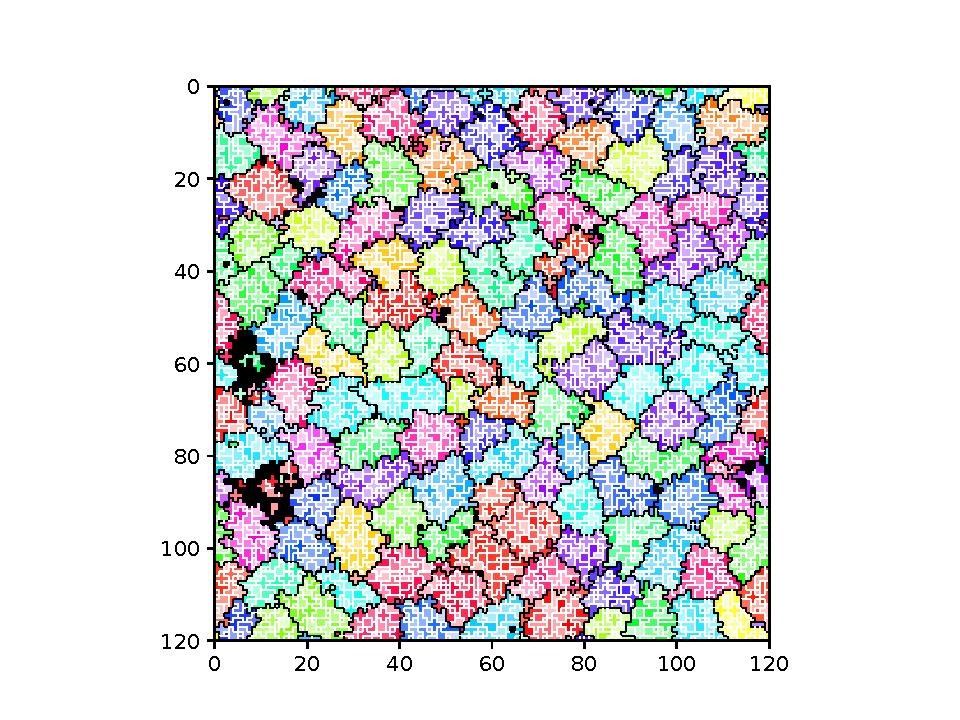
\includegraphics[width=\textwidth]{img/results/ChannelMap_1003_update24995104}
\end{column}
\begin{column}{0.4\textwidth}
\caption{
End state of same-channel signaling networks in simulation where exclusively level-one resource allocation dominated.
}
\end{column}
\end{columns}
\end{figure}
\end{frame}

\begin{frame}{Outcome: Intermediate Resource Allocation}
\begin{figure}
\begin{columns}
\begin{column}{0.6\textwidth}
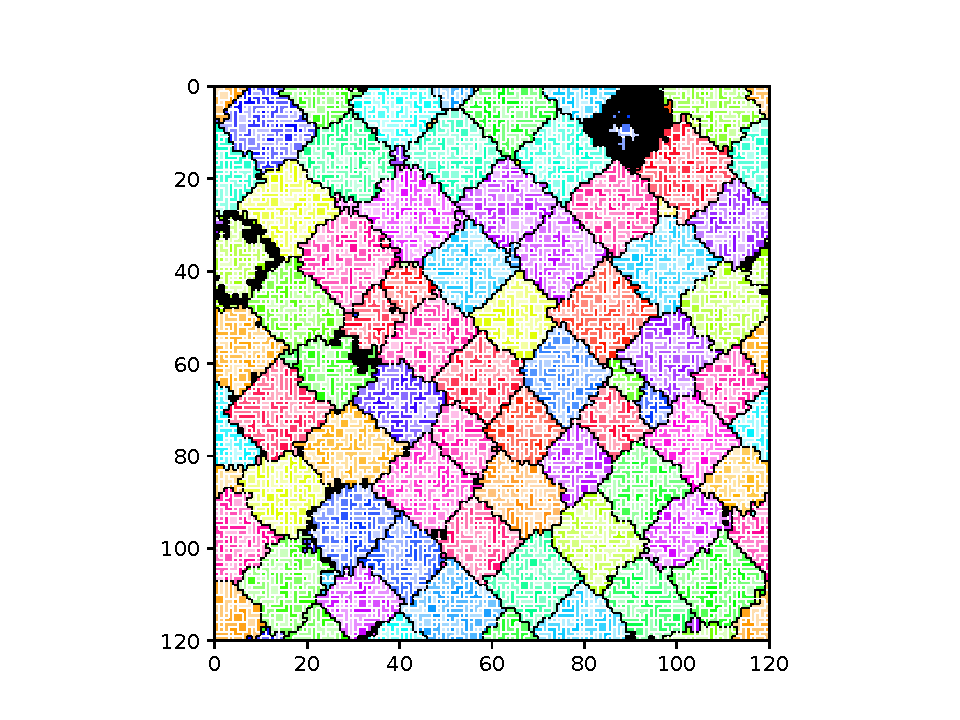
\includegraphics[width=\textwidth]{img/results/ChannelMap_1046_update24995104}
\end{column}
\begin{column}{0.4\textwidth}
\caption{
End state of same-channel signaling networks in simulation where intermediate resource allocation dominated.
}
\end{column}
\end{columns}
\end{figure}
\end{frame}

\begin{frame}{Outcome: Primarily Level 2 Resource Allocation}
\begin{figure}
\begin{columns}
\begin{column}{0.6\textwidth}
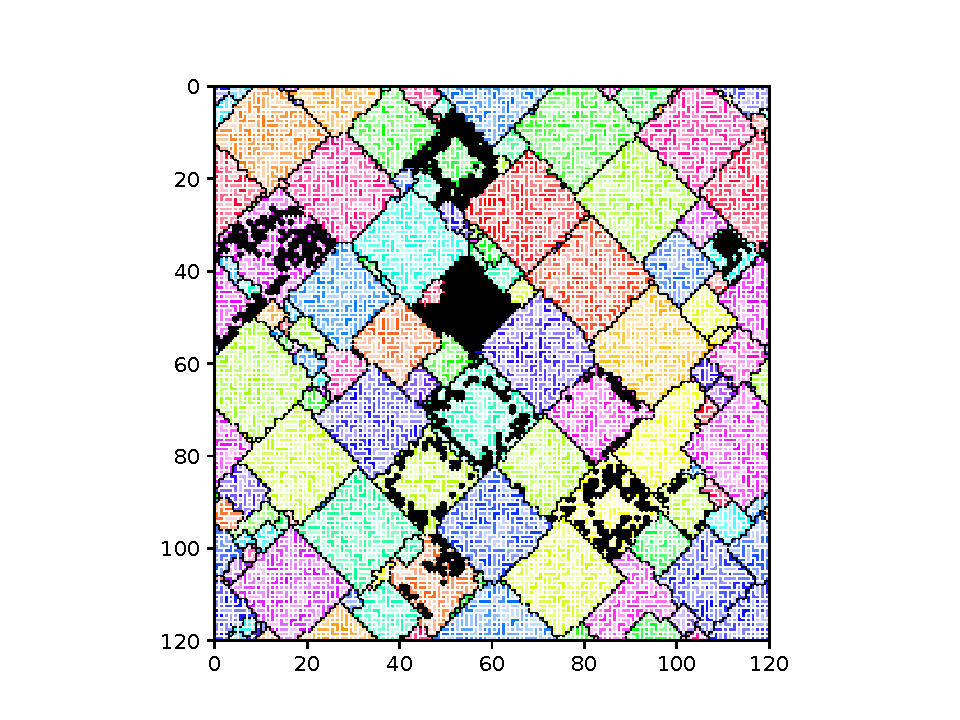
\includegraphics[width=\textwidth]{img/results/ChannelMap_1019_update24995104}
\end{column}
\begin{column}{0.4\textwidth}
\caption{
End state of same-channel signaling networks in simulation where primarily level-two resource allocation dominated.
}
\end{column}
\end{columns}
\end{figure}
\end{frame}

\begin{frame}{Level-one vs. Level-two Relative Fitness}

\begin{figure}
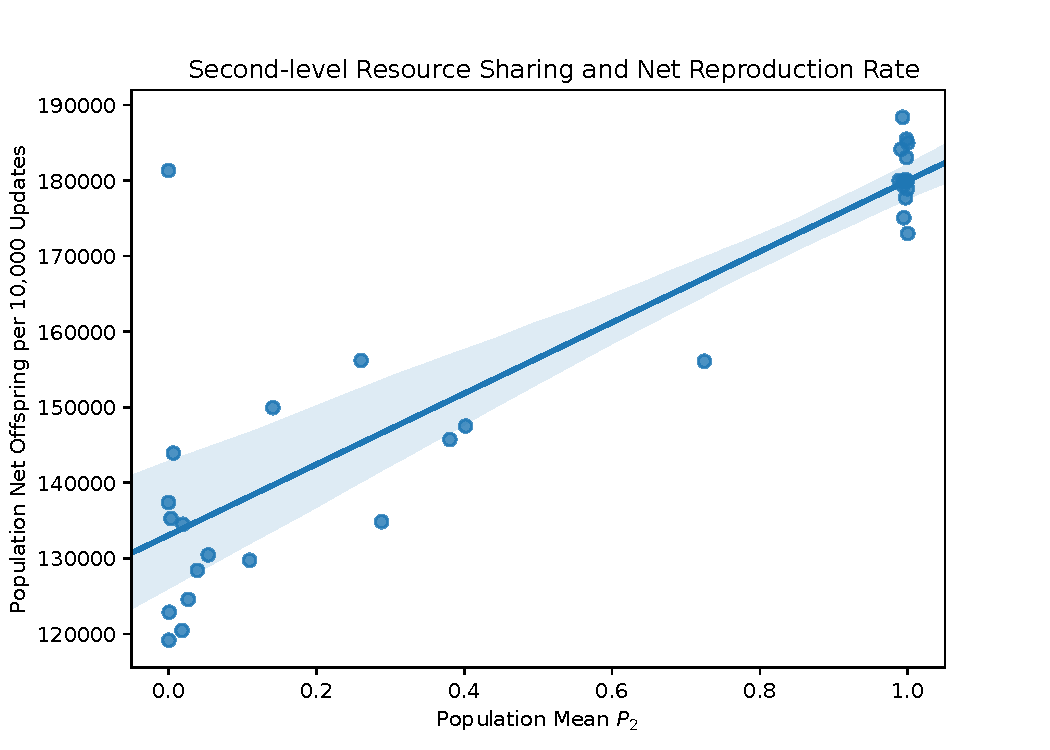
\includegraphics[width=0.8\textwidth]{results/mean_res_pool2_vs_net_reproduction}
\caption{
Correlation plot of population mean $P_2$ (resource-caching strategy) and population net reproduction rate.
A bootstrapped 95\% confidence interval for the fit is shaded.
}
\end{figure}

\end{frame}

\begin{frame}{Level-two Individuals' Apoptosis Response to Mutation}

\begin{figure}
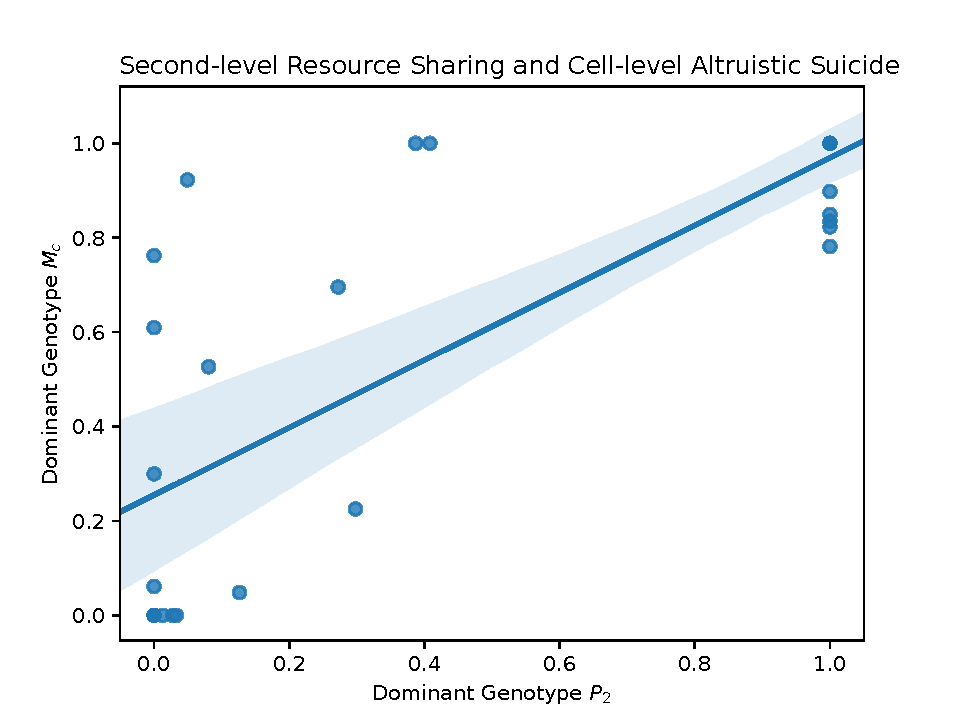
\includegraphics[width=0.8\textwidth]{results/champion_res_pool2_vs_champion_damage_suicide0}
\caption{
Correlation plot of dominant genotype $P_2$ (resource-caching strategy) and dominant genotype $M_{c}$ (apoptosis response to mutation).
A bootstrapped 95\% confidence interval for the fit is shaded.
}
\end{figure}

\end{frame}
